\begin{savequote}[10pc]
\sffamily
``Focus on people -- their lives, their work, their dreams.``
\qauthor{Google}
\end{savequote}

\lstset{language=Python}
\chapter{Interface for mobile devices}\label{chap:mobile}
In a context where the users of the application would rather be out surfing than
sitting home by their computer a mobile interface is essential. The application's
interface for mobile devices lets users access the weather service while on the
go. In this chapter, we describe the design and implementation of such an
interface for mobile devices, available at \url{http://m.welovewind.com/}.

In theory the mobile application could be situated at another domain, requesting
the data from the Web service over the network. However, since it is convenient
and faster to directly access the data models of the application we couple the
mobile interface to the Python data models, already presented.

%http://www.codeproject.com/KB/mobile/DeepCast.aspx
%http://www.skyhookwireless.com/devices/devicesupport.php  

\section{Design}
Most mobile devices have small screens, reduced computing power, reduced input
capabilities, and in general fewer functionalities than a standard computer. The
limitations mean that most mobile browsers are unable to render the standard
pages of the application since they rely on JavaScript; in addition, if they
could, the network latency and cost due to the size of the pages would be
significant. Therefore, the mobile version of the weather service calls for a
complete redesign and restructuring of the content, however, the overall
requirement is still the same: to present weather information that assist
practitioners of wind sports.

Figure~\ref{fig:mob_prototype} shows an early manifestation of the mobile user
interface: a user interface paper prototype. The prototype handles
Scenario~\ref{scenario:one} and Scenario~\ref{scenario:two}. Page number 1 on
the figure, is a form where the user must input his location by name. Since the
user most likely need information about the same location on the next visit, the
user's last entered location is automatically set in the form.

Users arrive at page 1 also when accessing the main URI with a mobile
device. Users therefore are relieved of 1) guessing the URI of the mobile page,
or if that is unsuccessful 2) using a search engine to find it.

The main content page of the mobile interface incorporates a concise version of
interesting location-based information, in a wind sports context. The page shows
spots in the proximity, weather observations from weather stations in the
proximity, and the weather forecast from the nearest forecast point. 

Page number 2 gives an all information about the current weather conditions. Page
4 is a map that shows spots and weather stations in the proximity of the
user. The map is important when the user needs to find the way to a new
spot. Page 3 and 5 are pages that show additional information about spots and
weather stations respectively.

\begin{figure}[htbp]
  \centering
  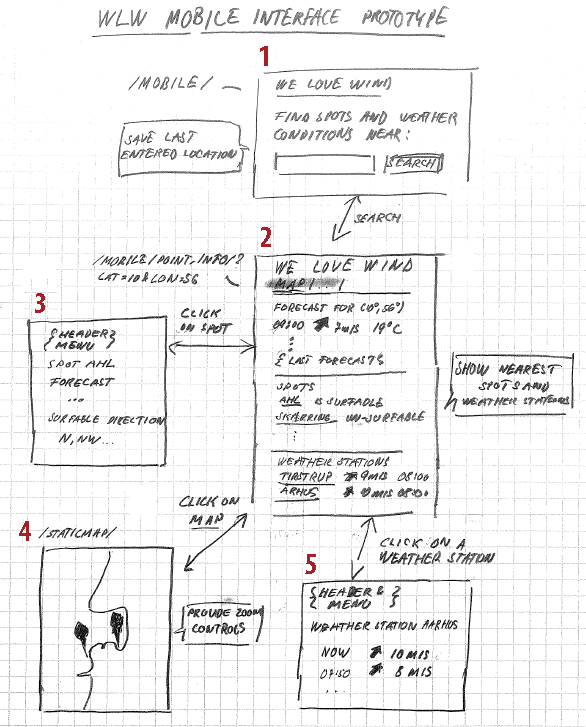
\includegraphics[width=12cm]{./Figures/mobile_prototype}
  \caption{Paper prototype of mobile interface}
  \label{fig:mob_prototype}
\end{figure}

The design discussed in the previous section adds four resources to the
application; the resources are shown in Table~\ref{tab:mobile_resources}. 

\begin{table}[htbp]
\centering \setlength\extrarowheight{3pt}
\begin{tabularx}{\textwidth}{l X X}
\toprule
Resource URI    & Query Parameters & Action\\\midrule
\verb|/mobile/|          & &\verb|GET| search page\\
\verb|/mobile/geo/|      & \verb|location| name &\verb|GET| geocoded location name\\
\verb|/mobile/info/|     & \verb|lat| latitude, 
                           \verb|lon| longitude, 
                           \verb|address| address & \verb|GET| all information for point\\
\verb|/mobile/map/|      & \verb|clat| latitude of center, 
                           \verb|clon| longitude of center,
                           \verb|zoom| zoom level of map,
                           \verb|spots| list of spot keys,
                           \verb|wss| list of weather station keys & \verb|GET| map with spots and weather stations centered around the given point\\
\bottomrule
\end{tabularx}
\caption{Resource view of mobile resources}\label{tab:mobile_resources}
\end{table}

\section{Sorting out the resource requirements}
In the last section we investigated the requirements and pointed out the
additional resources the requirements of the mobile client added to the Web
Service.  Some of the resource content requires somewhat non-trivial processing,
e.g., detecting a mobile client, displaying static maps apt for mobiles without
JavaScript, and converting times to a user relevant timezone. This section
reviews our solutions.

\subsection{Location-based mobile services}
Making a single location-based solution accessible for all browser clients
including mobile ones is impossible at the moment. 

More low level solutions like \citep{sun:lbs} exists, however, they rely on
technologies that are not ubiquitous either. We end up with a solution that rely
on mobile browsers rendering simple HTML pages with no JavaScript. More advanced
solutions could be developed, but the requirement is a widely accessible
solution. In addition, some of the advanced phones, e.g., iphone, are capable of
presenting the main page, see Figure~\ref{fig:iphone}. That is the mobile service
is a lowest common denominator solution.

\begin{figure}[htbp]
  \centering
  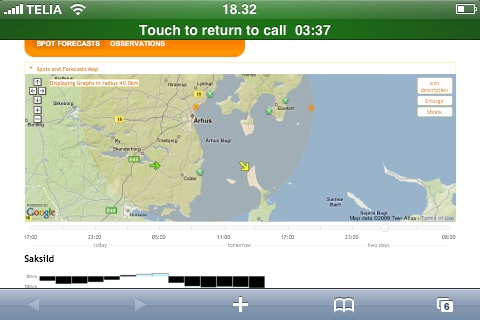
\includegraphics[width=10cm]{./Figures/iphone}
  \caption{Main page on iphone}
  \label{fig:iphone}
\end{figure}

\subsection{Content Negotiation}
Content negotiation is a term defined in \citep[sec.12]{w3:HTTP} which is a
mechanism to serve a representation of a resource based on the capabilities of
the client. In case of the application, users accessing the site with a mobile
should be served representations apt for mobile devices. All browsers populate
the user agent field in HTTP headers; this can be used to decide if the user is
accessing the site from a mobile device.

\begin{lstlisting}[caption=Mobile user agent detection, label=lst:mob_detection]
# special handling of theese
import logging
user_agents = ['ipod', 'android', 'opera mini', (...)]
# mobile user agents trimmed
more_user_agents = ['1207', '3gso', '4thp', '501i', (...)]

def mobile_device(request):
    '''Mobile device detection.
    
    Based on: 
        http://detectmobilebrowsers.mobi/
    Args:
        request: HTTP request
    Returns:
        bool indicating whether the user agent is a mobile device or not.
    '''
    # e.g., User-Agent: Opera/9.60 (J2ME/MIDP; Opera Mini/4.2.13918/422; U; da)
    user_agent = request.META['HTTP_USER_AGENT'].lower()
    logging.info('mobile.mobile_device: user_agent: %s' % user_agent)
    if 'iphone' in user_agent:
        return False
    for ua in user_agents:
        if user_agent.find(ua) != -1:
            return True
    if user_agent[0:4] in more_user_agents:
        return True
    return False
\end{lstlisting}

Listing~\ref{lst:mob_detection} shows the implementation, inspired by a PHP
implementation by \citep{mob:detection}, of user agent detection. The code contains
a list of mobile user agents and detects whether the user agent of the request is
one of them.

When the main page of the application is accessed the content negotiation is
performed. Listing~\ref{lst:cont_negotiation} shows how the root controller take
advantage of the content negotiation.  

HTTP caching is used to bypass the content negotiation on additional accesses to
the page from the same type of user agent.

\begin{lstlisting}[caption=Content negotiating controller,label=lst:cont_negotiation]
from wlw.helpers import mobile

from django import http

def index(request):
    '''Render the index page'''
 
    if mobile.mobile_device(request):
        response = http.HttpResponseRedirect('/mobile/')
    else:
        response = http.HttpResponseRedirect('/observations/')                                      
        response['Vary'] = 'User-Agent' # content varies by user-agent
        response['Cache-Control'] = 'public, max-age=604800' # cache for one week
    return response
\end{lstlisting}

\subsection{Local time}
In the Ajax client, JavaScript converted the UTC times of weather data served from
the Web Service to local times using the timezone of the user's machine. The
mobile interface must work without JavaScript demanding the time conversion to be
done at the server. There are three ways to realize the requirement for serving
time in a sensible timezone format:
\begin{itemize}
  \item let the user input timezone and save it as a cookie;
  \item associate user accounts with timezone information; or
  \item report times in the timezone where it applies.
\end{itemize}
The first and second demands the user to input timezone; whereas, the last
approach totally relieves the user for any input regarding the issue. Picking the
last solution, however, puts forth additional requirements of storing timezone
with all weather data owners: weather stations and forecast points. 

In Chapter~\ref{chap:gae_ws} the Forecast controller and Spot controller
retrieved timezone information from an external Web Service:
\url{http://www.geonames.org/}; it is now evident why: namely to realize option
number three. 

GeoNames is a free database containing extensive geographical
information. GeoNames provide access to its resources through different mainly
RESTful Web Services, and serves representations in XML and JSON formats. The
applied service is the timezone service.

The implementation of code that retrieves a timezone from a point from GeoNames
is shown in Listing~\ref{lst:geonames_tz}. The code uri-encodes the point, fetches
the resource, and handles different failures.

\begin{lstlisting}[caption=Using GeoNames timezone Web Service, label=lst:geonames_tz]
def geonames_timezone(point):
    '''Get timezone information with geonames.org.
    
    Returns:
        json string {'time':..., 'countryName': ..., 'countryCode':..., 'timezoneid': ...}
    '''
    values = {'lat':point.lat, 'lng':point.lon}
    query = http.urlencode(values)
    timezone_uri = 'http://ws.geonames.org/timezoneJSON?%s' % query
    try:
        response = urlfetch.fetch(url=timezone_uri)
        if response.status_code != 200:
            raise WSException('geonames.org not available')
        if 'message' in response.content:
            json = simplejson.decode(response.content)
            raise WSException('ws.geonames.org: %s' % json['status']['message'] )
        return response
    except DownloadError, e:
        raise WSException('geonames.org not available')
\end{lstlisting}

With the timezone in place the times are converted with the logic presented in
Section~\ref{sec:gae_tz}.


\subsection{Geocoding}
Geocoding is applied in order to map from the user input location names to a
latitude and longitude location. There are several geocoding services:
Yahoo\footnote{http://local.yahooapis.com/MapsService/V1/geocode},
GeoNames\footnote{http://www.geonames.org/export/geonames-search.html}, and
\citep{google:geo}.

GeoNames is free, however, the author has experienced low availability of the Web
service. Yahoo, restricts the number of geocoding requests to 5000 pr. day pr. IP
address. Google restricts their service to uses that includes displaying markers
on a Google map. The Google \gls{gls:geocoding} service is chosen, since the mobile
interface presents markers on a Google map. 

Listing~\ref{lst:google_geo} shows how the service is put to use from GAE. The
code takes the following sequence of steps:
\begin{itemize}
  \item Builds an URI to the Google Web service to query. 
  \item Handles different failures, and throw a custom exception if so.
  \item Decodes and inserts the JSON response into a data structure.
  \item Uses memcache to bypass the \gls{gls:geocoding} service, and speed up
additional requests for the same location.
\end{itemize}

\begin{lstlisting}[caption=Google geocoding in Python, label=lst:google_geo]
def google_geocode(location):
    '''Geocode by location name.
    Args:
        location: name of location.
    Returns:
        location info as dictionary {'lat':..., 'lon':...,'address':...}
    '''
    data = memcache.get('/geo/location/%s' % location)
    if data is not None:
        return data 
    else:
        values = {'key': settings.GOOGLE_APP_ID,'q': location, 'output':'json', 'oe':'utf8', 'sensor': 'false'}
        query = http.urlencode(values)
        geocoding_uri = 'http://maps.google.com/maps/geo?%s' % query
        response = urlfetch.fetch(url=geocoding_uri)
        if response.status_code != 200:
            raise WSException('Error finding location')
        json = simplejson.loads(response.content)
        status_code = json['Status']['code']
        if status_code >= 500:
            raise WSException('Could not find location')
        placemark = json['Placemark'][0]
        lat = float(placemark['Point']['coordinates'][1])
        lon = float(placemark['Point']['coordinates'][0])
        address = placemark['address']

        data = {'lat':lat,'lon':lon, 'address':address} 
        if lat and lon and address:
            memcache.add('/geo/location/%s' % location, data)
        return data
\end{lstlisting}

\subsection{Displaying static Google maps}
Google Static
Maps\footnote{\url{http://code.google.com/apis/maps/documentation/staticmaps/}} is a
Web Service that takes an HTTP request generates a static map images and responds
with the image. The service is useful in a context where JavaScript is
unavailable such as our mobile service.

It is easy to put the Static Maps Web Service to use, e.g., retrieving a map of
Denmark is done by issuing a request to the URI:
\begin{verbatim}
http://maps.google.com/staticmap?center=56,10&zoom=6&size=512x512&
        maptype=mobile&sensor=false  
\end{verbatim}
Since the representation format is an image format the URI can be placed in a
usual \verb|img| tag in HTML documents.
\begin{verbatim}
<img src="http://maps.google.com/staticmap?center=56,10&
zoom=6&size=512x512&maptype=mobile&sensor=false />  
\end{verbatim}
Markers on the static map are specified by defining a list of marker descriptors
and setting them as the value of the URI parameter \verb|markers|. A URI
parameter such as
\begin{verbatim}
...&markers=56,10,blue1|57,10,blue2&...
\end{verbatim}
indicates a resource with two marker descriptors that each contains a blue marker
at a specified point. It is possible to suffix marker colors with a single
character that is shown inside the marker, in this case \verb|1| and \verb|2|,

The application dynamically creates the relevant URIs to a static map resource,
and inserts them into the mobile map page. Listing~\ref{lst:gsmaps_creator} shows two
functions: \verb|create_static_markers| and \verb|gsmap_uri|. The former method
takes any list of points and converts them to an appropriate string with a list
of marker descriptors. The latter sets relevant parameters, uri-encodes them, and
returns the URI to the static map resource.

\begin{lstlisting}[caption=Google Static Maps URI creator,label=lst:gsmaps_creator]
def gsmap_uri(center, markers, zoom=8):
    '''Get the URI of the Static Google Map.
    
    Args:
        zoom: the zoom level.
        markers: string with a list of marker descriptors to put on the map.
    Returns:
        the URI of the map resource.
    '''
    values = {
        'size': '200x200',
         # precision of points is 6 decimals
        'center': '%s,%s' % (round(center.lat,6), round(center.lon,6)),
        'maptype':'mobile',
        'markers': markers,
        'key':settings.GOOGLE_APP_ID,
        'sensor':'false',
        'format':'jpg',
        'zoom':zoom
        }
    query = urlencode(values)
    return 'http://maps.google.com/staticmap?%s' % (query)

characters = '123456789abcdefghijklmnopqrstuvwxyz'
   
def create_static_markers(places, color = ''):
    '''Create markers for Google Static Maps API.
    
    Args:
        places: list of points
        color: ('black'| 'brown'| 'green'| 'purple'| (...)
    Returns:
        a string of markers like "10,50,blue1|10,55,blue2".
    '''
    markers = []
    for index, p in enumerate(places):
        marker = '%s,%s,%s' % (round(p.point.lat, 6), round(p.point.lon, 6), color)
        if index < len(characters):
            marker += '%s' % (characters[index])
        markers.append(marker) 
    return '|'.join(markers)
\end{lstlisting}


\section{Implementation}
The implementation is a typical server side Web application: on requests the
server assembles a HTML page and sends it to the client. 

\subsection{Controllers}
The requirements for the mobile application yield four new resources. We skip
presenting the regular expressions, mapping URIs to controller methods, and jump
directly to the implementation of the controllers.

\subsubsection{Search and Geo controller}
The Geo controller handles \gls{gls:geocoding} of the location names
input by the user on the search page. After a successful geocoding the controller
saves the result in a cookie, which enable the last location to automatically be
presented on additional visits to the search page. We skip the code for the
search controller since it only checks for the presence of the cookie, and
renders the search form. 

With the geocoder in place the controller is left off handling exceptions and
setting the cookie. The geocoded address is converted to a byte string before
setting it as a cookie since they can only contain ascii data. After a successful
geocode the controller returns a redirect to the info resource.

\begin{lstlisting}[caption=Geo controller, label=lst:geo_controller]
  def geo(request):
    location = request.GET.get('location', None)
    if location is None:
        http.HttpResponseBadRequest('location must be set')
    try:
        geo = geoinfo.google_geocode(location)
        query = urlencode(geo)
        r = http.HttpResponseRedirect('/mobile/info/?%s' % (query))
        # 2592000 sec. = 1 month
        r.set_cookie('latest_address', smart_str(geo['address']), max_age=2592000)
        return r
    except WSException, e:
        return http.HttpResponse(e)
\end{lstlisting}

\subsection{Map Controller}
Static maps are presented by the map controller. The resource is a typical
algorithmic resource where the uri-parameters can be seen as input into an
algorithm that creates a map. 

The map controller takes as input the latitude and longitude of the center of the
map, and a list of spot and weather station keys, representing points to put on
the map. Point entities are retrieved from the datastore by directly giving them
as a list to the datastore method \verb|get_by_key_name|.

The controller rely on the functions in the \verb|gstaticmaps| module to create
the URI for the static map resource on Google. The controller maintains many
uri-parameters to handle the \textit{\gls{gls:appstate}}, and keeping the server
stateless. An example is the \verb|zoomed| query dictionary that contains a
complete copy of the uri-parameters only deviating on the value of \verb|zoom|.

\begin{lstlisting}
def map(request):
    '''The map page
    
    Args GET:
        clat: center latitude of map
        clon: center longitude of map
        spots: spotkey1;spotkey2;...
        wss: wskey1;wskey2;...
        zoom: the zoom level of the map
    '''
    center_lat = request.GET['clat']
    center_lon = request.GET['clon']
    zoom = int(request.GET.get('zoom', 8))        
    spot_keys = request.GET.get('spots', None)
    wss_keys = request.GET.get('wss', None)
        
    spots, wss = [], []
    if spot_keys:
        spots = Spot.get_by_key_name(spot_keys.split(';'))
    if wss_keys:
        wss = WeatherStation.get_by_key_name(wss_keys.split(';'))

    query_dict = request.GET.copy()
    # zoom in
    query_dict['zoom'] = zoom + 2
    zoomed = query_dict.urlencode()
    # zoom out
    query_dict['zoom'] = zoom - 2 
    zoomed_out = query_dict.urlencode()
    
    spot_markers = gstaticmaps.create_static_markers(spots, 'blue')
    wss_markers = gstaticmaps.create_static_markers(wss, 'green')
    markers = '|'.join([spot_markers, wss_markers])
    
    static_map_uri = gstaticmaps.gsmap_uri(
        db.GeoPt(lat=center_lat, lon=center_lon), markers, zoom)
    
    address = request.GET.get('address')
    
    values = {
        'lat': request.GET.get('lat'),
        'lon': request.GET.get('lon'),
        'address': address}
    
    qs = urlencode(values)
    
    return shortcuts.render_to_response(
        'map_mobile.xhtml',
        {'spots':spots, 'wss':wss, 'static_map_uri':static_map_uri, 'qs': qs,
            'qs_zoomed': zoomed, 'qs_zoomed_out':zoomed_out}        
    )
\end{lstlisting}

\subsection{Info controller}
The info controller provides access to the main mobile content page: page 2 in
the prototype. From a given geographic point the controller retrieves all weather
stations and spots within a 50 km radius, by using the \verb|get_near_point|
method presented in Section~\ref{sec:models}; the method sorts the points by
distance raising the relevance of the first presented points, of each category,
in the user interface. The length of the geohash prefix, input to
\verb|get_by_distance| was chosen on a pure pragmatic basis using the geohash
demonstrator.\footnote{\url{http://www.welovewind.com/examples/geohash/index.html}}

\begin{lstlisting}
def info(request):
    '''Info about a point.
    
    Retrieve spots, weather stations in the proximity, and the forecasts for the point.
    
    Args GET:
        lat: latitude of point
        lon: longitude of point
        address: address of point
    '''
    lat = float(request.GET.get('lat'))
    lon = float(request.GET.get('lon'))
    if lat is None or lon is None:
        http.HttpResponseBadRequest('lat/lon must be set')
    address = request.GET.get('address', '(%s,%s)' % (lat, lon))
    
    center = db.GeoPt(lat=lat, lon=lon)
    
    wss = WeatherStation.get_by_point(center, 50, 3)
    spots = Spot.get_by_point(center, 50, 3)
    forecast_point = ForecastPoint.get_or_init_by_point(center)
    
    spot_keys = [s.key().name() for s in spots]
    wss_keys = [w.key().name() for w in wss]
    
    # the 'list' is just a key string separated by commas in the uri.
    map_values = {
        'clat': lat,
        'clon': lon,
        'spots': ';'.join(spot_keys),
        'wss': ';'.join(wss_keys),
    }
    
    map_uri = '/mobile/map/?%s' % urlencode(map_values)
    
    return shortcuts.render_to_response(
        'info_mobile.xhtml',
        {
            'map_uri':map_uri,
            'spots':spots,
            'wss':wss,
            'fp':forecast_point,
            'qs': request.GET.urlencode(),
            'address': address
        })
\end{lstlisting}


\subsection{Views}
% http://www.w3.org/TR/mobile-bp/
All the views of the mobile interface are valid XHTML Basic 1.1: the W3C
recommendation for content the format for mobile interfaces
\citep{w3c:mobile}. We skip presenting the views of the mobile application. The
interested reader can refer to Appendix~\ref{app:mobile} for the views.

\section{Summary}
In this chapter, we extended the application with a mobile interface, to support
scenarios where the user is on the go. The mobile interface had a significant
impact on the application in terms of complexity. The added complexity stems from
1) a requirement for the mobile application being widely accessible, and 2) the
limit of many mobile browsers. The application could not rely on JavaScript, and
therefore functionality already developed in JavaScript, such as timezone
conversion and display of maps, was implemented on the server side also.
